\subsection{STAN: Towards Describing Bytecodes of Smart Contract}
\label{subsec:stan}

Penelitian yang dilakukan oleh \cite{stan} mengusulkan sebuah sistem bernama STAN untuk melakukan deskripsi terhadap \textit{bytecodes} dari Smart Contracts. STAN merupakan sebuah sistem yang dirancang untuk mengatasi masalah dalam mengekstraksi informasi dari \textit{bytecodes} yang dihasilkan oleh kompilator Solidity. Untuk setiap \textit{interface}, terdapat empat kategori deskripsi yang dapat dihasilkan, yaitu: \textit{functionality description}, \textit{usage description}, \textit{behaviour description}, dan \textit{payment description}. STAN bekerja dengan memanfaatkan \textit{symbolic execution} dan \textit{Natural Language Processing} (NLP) untuk menghasilkan deskripsi yang lebih mudah dipahami oleh pengguna.

\begin{figure}[ht]
  \centering
  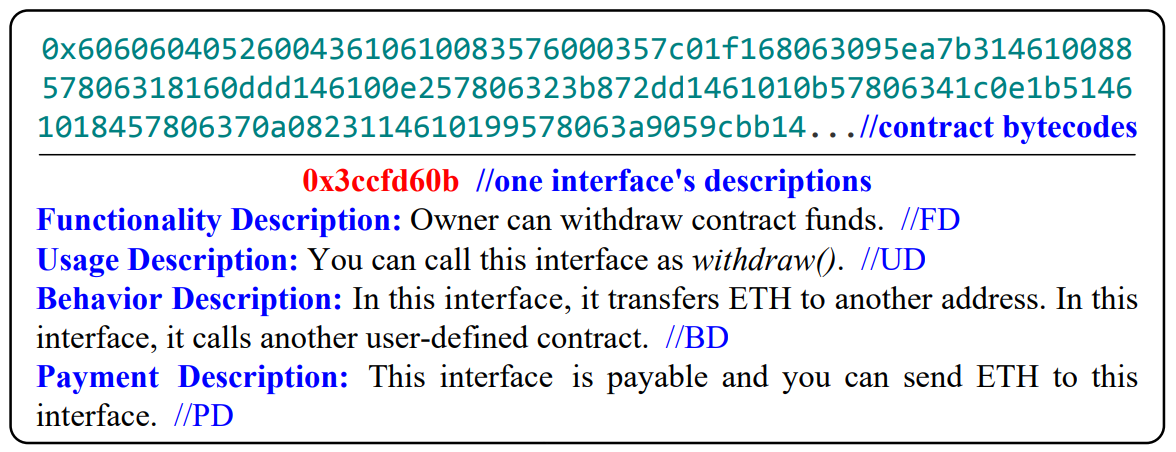
\includegraphics[width=0.7\textwidth]{resources/chapter-2/stan-desc.png}
  \caption{Hasil deskripsi dari STAN untuk Bytecode salah satu \textit{closed-source} Smart Contract \parencite{stan}}
  \label{image:stan-desc}
\end{figure}

\begin{figure}[ht]
  \centering
  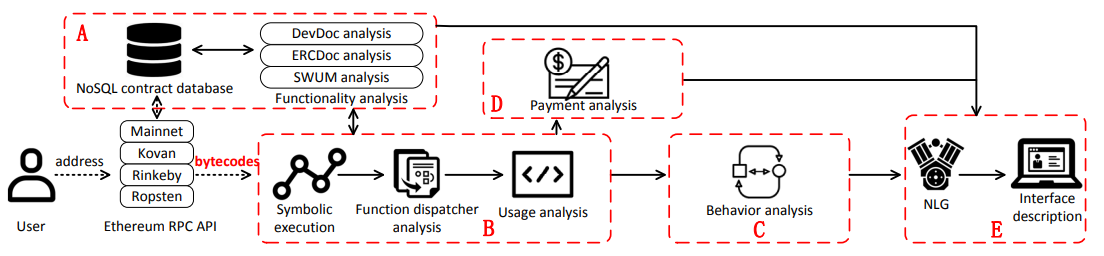
\includegraphics[width=0.7\textwidth]{resources/chapter-2/stan-architecture.png}
  \caption{Arsitektur sistem STAN \parencite{stan}}
  \label{image:stan-architecture}
\end{figure}

Arsitektur dari STAN (Gambar \ref{image:stan-architecture}) terdiri dari beberapa modul utama, yaitu:

\begin{enumerate}
  \item \textbf{Functionality Analysis Module} \\
  Modul ini melakukan analisis terhadap kontrak melalui teknik \textit{Natural Language Processing} (NLP) untuk menghasilkan frasa yang terkait dengan fungsionalitas dari \textit{interface} kontrak. Fungsionalitas utama dari modul ini adalah untuk mendeskripsikan Bytecode \textit{closed-source contracts}, sementara kontrak \textit{open-source contracts} dan metadata dianalisis untuk membantu analisis Bytecode dengan menemukan \textit{byte signatures} yang identik.

  \item \textbf{Usage Analysis Module} \\
  Modul ini mengekstrak \textit{byte signatures} fungsi dari \textit{dispatcher} fungsi dan mengembalikan \textit{signature} teks yang sesuai. Dari \textit{signature} teks (misalnya \texttt{transfer(address, uint256)}), pengguna dapat mengetahui nama fungsi dan konfigurasi parameter yang digunakan untuk memanggil \textit{interface}. Modul ini memungkinkan pemahaman yang lebih baik mengenai bagaimana fungsi digunakan dalam kontrak.

  \item \textbf{Behavior Analysis Module} \\
  Modul ini menganalisis fungsi eksternal/publik untuk menghasilkan informasi perantara terkait perilaku panggilan pesan menggunakan \textit{symbolic execution}. Dengan menganalisis opcode dan operand, modul ini dapat mengenali empat jenis perilaku sensitif dalam panggilan pesan, seperti transfer ETH, penerapan kontrak, dan panggilan kontrak.

  \item \textbf{Payment Analysis Module} \\
  Modul ini menganalisis fungsi eksternal/publik untuk menghasilkan informasi perantara terkait fitur pembayaran melalui \textit{symbolic execution}. Dengan membangun \textit{Control Flow Graph} (CFG), modul ini dapat mengenali dua pola pembayaran yang menunjukkan apakah \textit{interface} tersebut dapat melakukan pembayaran atau tidak.

  \item \textbf{NLG Module} \\
  Modul ini menghasilkan deskripsi \textit{interface} yang dapat dibaca dengan memanfaatkan hasil dari empat modul sebelumnya. Proses \textit{Natural Language Generation} (NLG) mengikuti alur standar sistem NLG, yaitu \textit{document planner}, \textit{microplanner}, dan \textit{surface realizer}, untuk menghasilkan deskripsi \textit{interface} yang mudah dipahami oleh pengguna.
\end{enumerate}

STAN dikembangkan pada tahun 2020, dan mencapai hasil yang sangat baik dalam melakukan deskripsi Smart Contract yang bersifat \textit{closed-source}, yang meliputi sekitar 99\% dari seluruh Smart Contracts. Dengan adanya STAN, pengguna dapat memahami fungsionalitas, penggunaan, perilaku, dan pembayaran yang terkait dengan Smart Contract tanpa harus melihat kode sumber dari kontrak tersebut. Hasil deskripsi dari STAN dapat dilihat pada Gambar \ref{image:stan-desc}. STAN adalah sebuah perangkat lunak yang tidak bersifat \textit{open-source} sehingga tidak dapat digunakan secara luas. Namun, konsep yang diusulkan oleh STAN dapat dijadikan sebagai dasar untuk pengembangan sistem yang serupa.
